\chapter{Các khái niệm \& định luật cơ bản}
\section{Giới hạn và phạm vi ứng dụng của bài toán mạch }
\section{Các phần tử mạch}
\textbf{Mạch điện:} là một hệ gồm các thiết bị điện, điện tử được gắn kết với nhau bằng dây dẫn thành vòng kín trong đó xảy ra các quá trình truyền đạt, biến đổi năng lượng hay các tín hiệu điện từ.
\begin{center}
  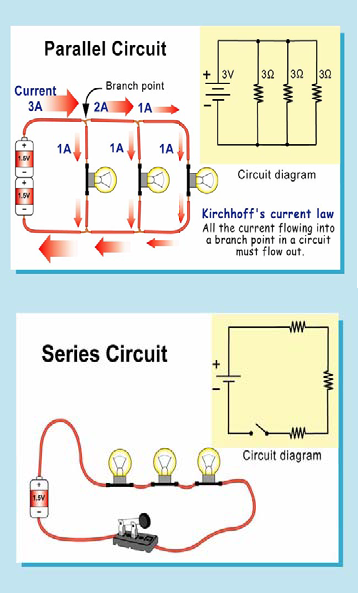
\includegraphics[width=0.35\textwidth]{./image/1(1).png} \quad \quad \quad \quad 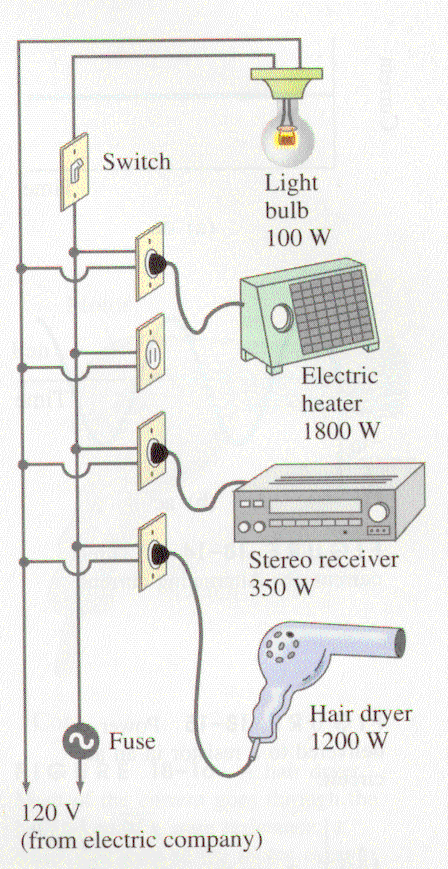
\includegraphics[width=0.35\textwidth]{./image/1(2).png}
\end{center}
\begin{center}
  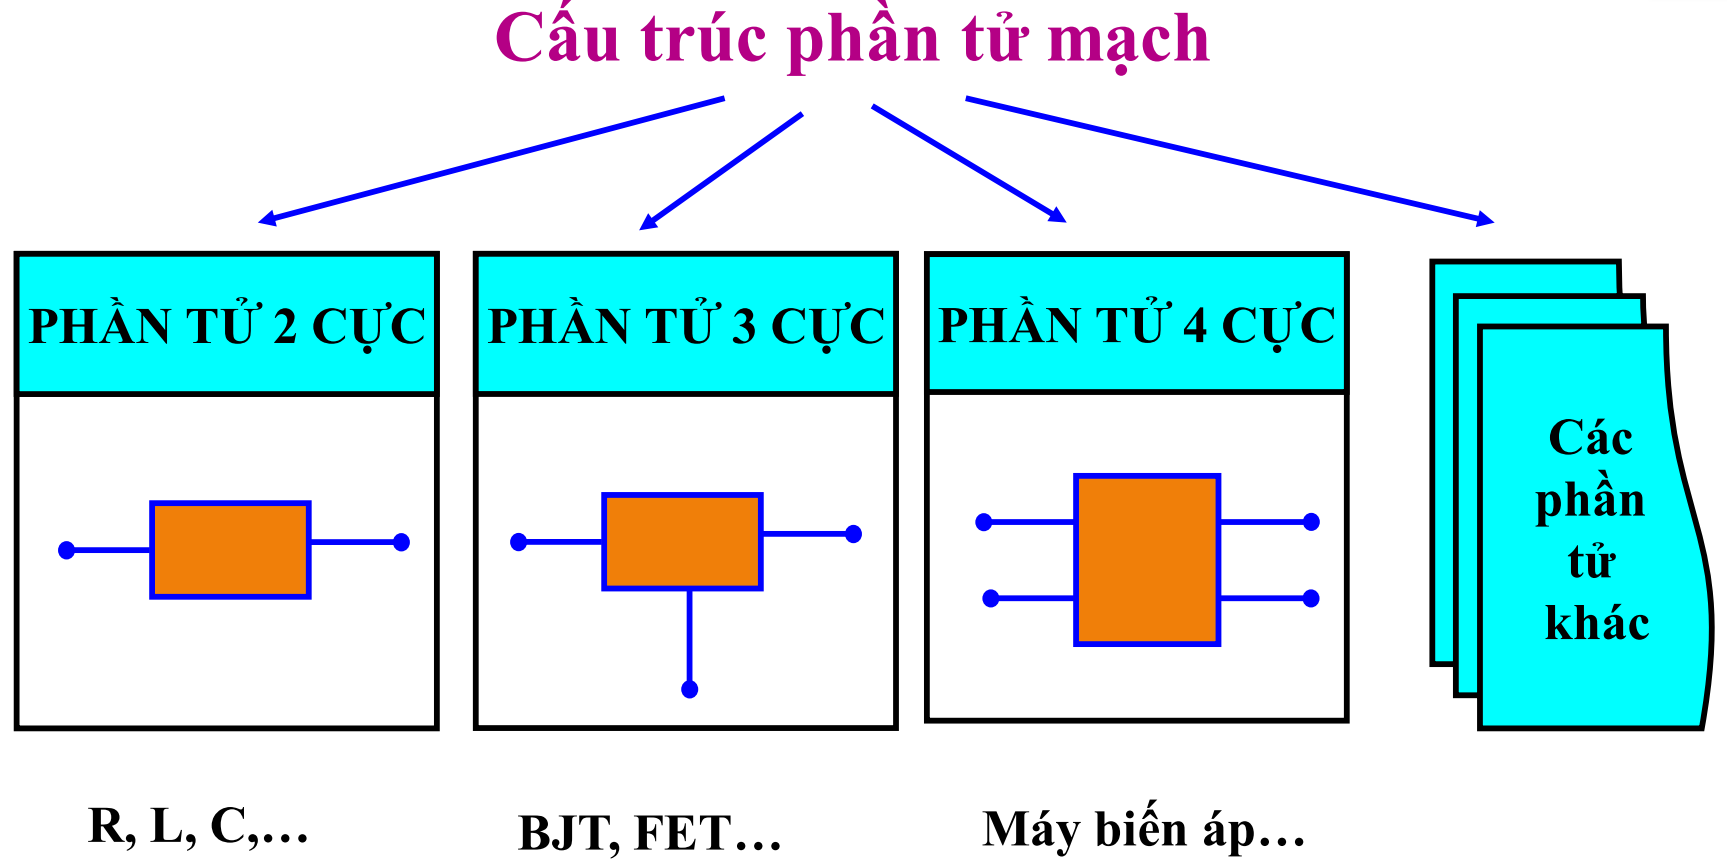
\includegraphics[width=0.8\textwidth]{./image/2.png}
\end{center}
\subsection{Điện trở}
\begin{itemize}
  \item Đặc trưng cho tổn hao công suất trong mạch điện.
  \item Quan hệ dòng áp trên 2 cực theo định luật Ohm:
    \begin{equation}
      u(t) = Ri(t)
    \end{equation}
  \item $R$: điện trở đơn vị Ohm ($\Omega$). Ký hiệu trong sơ đồ:
\end{itemize}
\begin{center}
  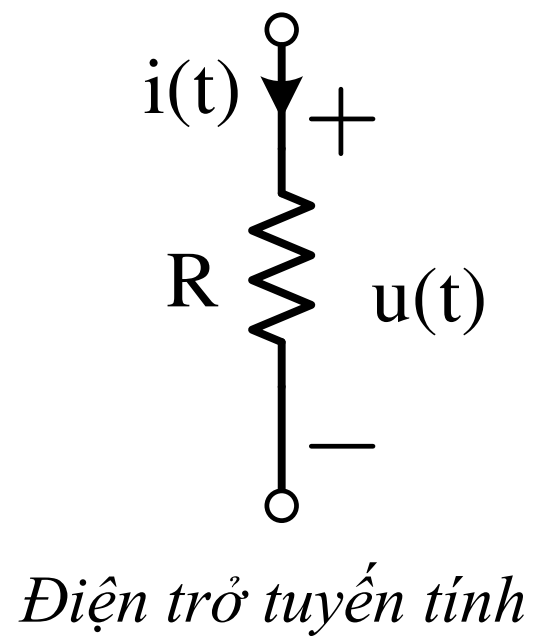
\includegraphics[width=0.25\textwidth]{./image/3.png} \quad \quad \quad 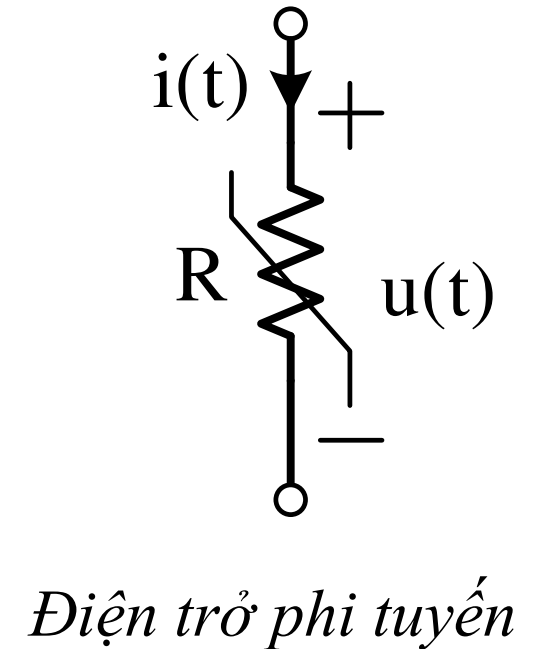
\includegraphics[width=0.25\textwidth]{./image/4.png}
\end{center}
\subsection{Điện cảm}
\begin{itemize}
  \item Đặc trưng cho tích phóng năng lượng từ trường.
  \item Quan hệ dòng áp trên điện cảm tuyến tính:
  \begin{equation}
    u_L(t) = L\frac{di_L(t)}{dt} \hspace{1in} i_L(t)=\frac{1}{L}\int_{t_0}^{t} u_L(t)dt 
  \end{equation}
  \item $L$: điện cảm (độ tự cảm) đơn vị Henry (H). Ký hiệu trong sơ đồ
\end{itemize}
\begin{center}
  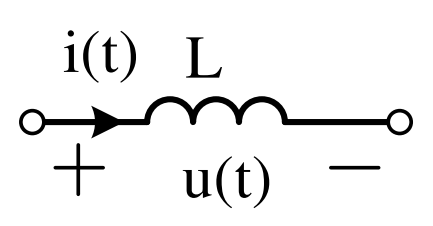
\includegraphics[width=0.25\textwidth]{./image/5.png}
\end{center}
\subsection{Điện trường}
\begin{itemize}
  \item Đặc trưng cho tích phóng năng lượng điện trường.
  \item Quan hệ dòng áp trên điện dung tuyến tính:
    \begin{equation}
      i_C(t) = C\frac{du_C(t)}{dt} \hspace{1in} u_C(t)=\frac{1}{C}\int_{t_0}^{t} i_C(t)dt 
    \end{equation}
  \item $C$: điện dung đơn vị Fara (F). Ký hiệu trong sơ đồ
\end{itemize}
\begin{center}
  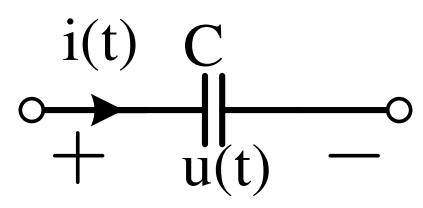
\includegraphics[width=0.25\textwidth]{./image/6.png}
\end{center}
\subsection{Hỗ cảm}
\begin{itemize}
  \item Là hiện tượng xuất hiện từ trường trong cuộn dây do dòng điện trong cuộn dây khác tạo nên.
\end{itemize}
\begin{equation}
  \Psi_{11} = L_1i_1,\ \Psi_{22} = L_2i_2 \Rightarrow 
  \begin{cases}
    u_1 = \pm\dfrac{d\Psi_{11}}{dt}\pm\dfrac{d\Psi_{12}}{dt} \\ \\
    u_2 = \pm\dfrac{d\Psi_{22}}{dt}\pm\dfrac{d\Psi_{21}}{dt} 
  \end{cases}
\end{equation}
\begin{itemize}
  \item Hệ số hỗ cảm: $M = \dfrac{\Psi_{21}}{dt} = \dfrac{\Psi_{12}}{dt}$
  \item Mức độ ghép giữa 2 cuộn dây xác định thông qua hệ số $k$. $k = \dfrac{M}{\sqrt{L_1L_2}},\ 0<k<1$.
\end{itemize}
\begin{center}
  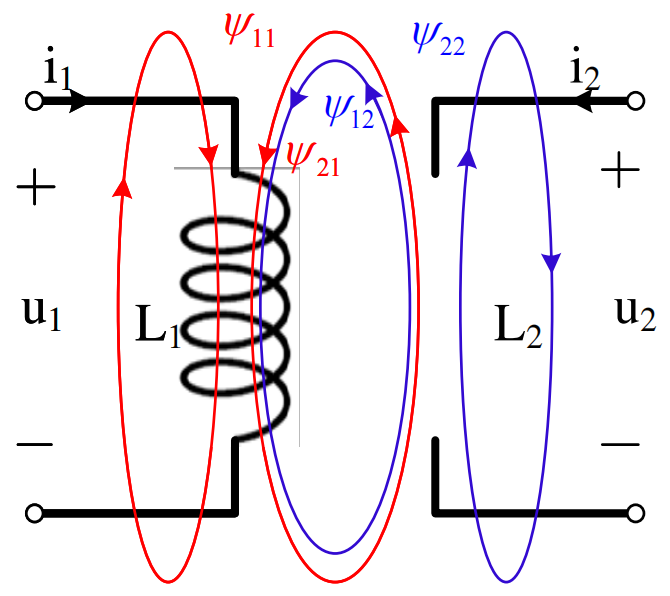
\includegraphics[width=0.35\textwidth]{./image/7.png}
\end{center}
\begin{equation}
  \begin{cases}
    u_1 = \pm L_1\dfrac{di_1}{dt}\pm M\dfrac{di_2}{dt} \\ \\
    u_2 = \pm L_2\dfrac{di_2}{dt}\pm M\dfrac{di_1}{dt}
  \end{cases}
\end{equation}
Trong đó:
\begin{itemize}
  \item $\pm L_1\dfrac{di_1}{dt},\ \pm L_2\dfrac{di_2}{dt}$: Xét dấu theo chiều dòng điện đang chảy trong cuộn dây đối với chiều sụt áp.
  \item $\pm M\dfrac{di_2}{dt},\ \pm M\dfrac{di_1}{dt}$: Xét dấu theo vị trí các cực cùng tên đối với chiều các dòng điện.
\end{itemize}
VD:
\begin{center}
  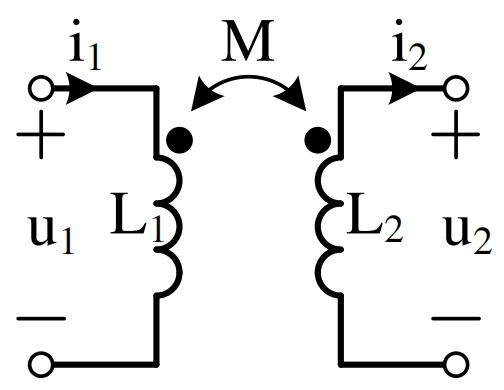
\includegraphics[width=0.35\textwidth]{./image/8.png}
\end{center}
\[
  u_1 = +L_1\dfrac{di_1}{dt}- M\dfrac{di_2}{dt},\ u_2 = - L_2\dfrac{di_2}{dt}+ M\dfrac{di_1}{dt}
\]
\subsection{Nguồn áp}
\textbf{Nguồn áp độc lập:}
\begin{itemize}
  \item Với quan hệ $u(t) = e(t)$. 
  \item Trong đó $u(t)$ không phụ thuộc dòng điện $i(t)$ cung cấp từ nguồn và chính bằng sức điện động của nguồn.
\end{itemize}
\begin{center}
  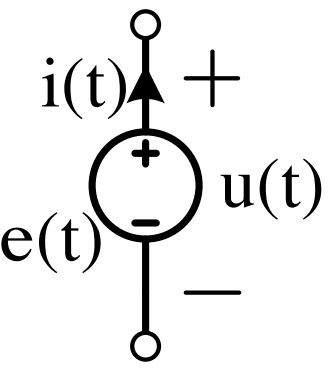
\includegraphics[width=0.2\textwidth]{./image/9.png}
\end{center}
\textbf{Nguồn áp phụ thuộc:} $u(t)$ quan hệ phụ thuộc theo áp hoặc dòng trên một nhánh khác.
\begin{center}
  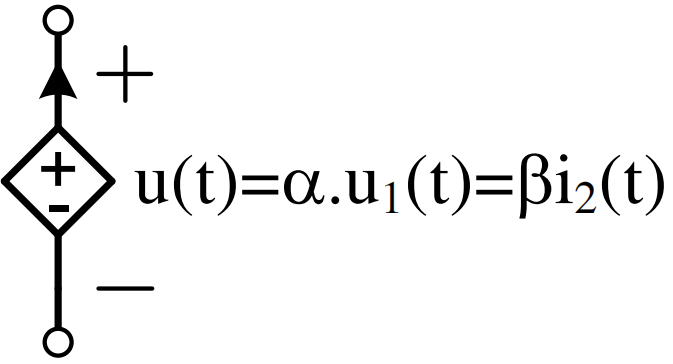
\includegraphics[width=0.35\textwidth]{./image/10.png}
\end{center}
\subsection{Nguồn dòng}
\textbf{Nguồn dòng độc lập:} 
\begin{itemize}
  \item Với quan hệ $i(t)=j(t)$.
  \item Trong đó $i(t)$ không phụ thuộc vào điện áp $u(t)$.
\end{itemize}
\begin{center}
  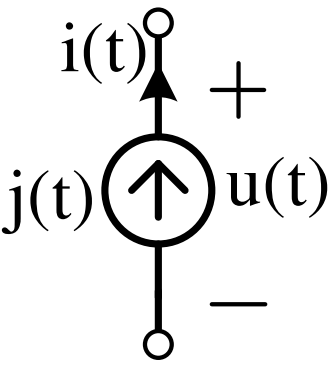
\includegraphics[width=0.2\textwidth]{./image/11.png}
\end{center}
\textbf{Nguồn dòng phụ thuộc:} $i(t)$ quan hệ phụ thuộc theo áp hoặc dòng trên một nhánh khác.
\begin{center}
  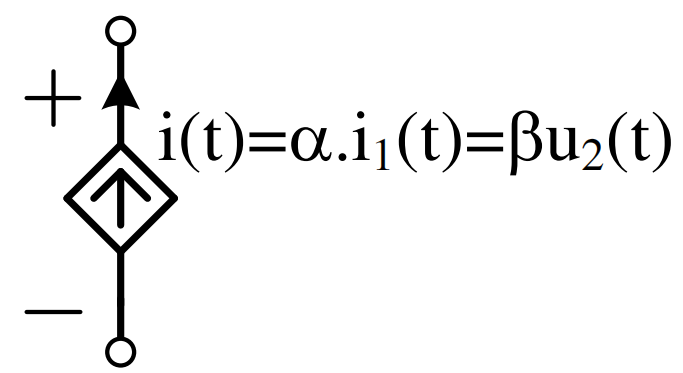
\includegraphics[width=0.35\textwidth]{./image/12.png}
\end{center}
\section{Công suất và năng lượng}
\subsection{Công suất}
\noindent Công suất tức thời: 
\begin{equation}
  p(t)=u(t).i(t)
\end{equation}
Công suất trung bình: 
\begin{equation}
  P= \frac{1}{T}\int_{t_0}^{t_0 + T} p(t)dt \qquad \lbrack W\rbrack
\end{equation}
\subsection{Năng lượng}
\noindent Năng lượng được hấp thu bởi phần tử mạch trong khoảng vô cùng bé $dt$ được xác định bởi:
\begin{equation}
  dW = udq = u.i.dt
\end{equation}
Năng lượng hấp thu bởi mạch trong khoảng thời gian $t_0$ + $t_0 + \Delta t$
\begin{equation}
  W = \int_{t_0}^{t_0 + \Delta t} u.i.dt \qquad \lbrack J\rbrack
\end{equation}
\begin{table}[h!]
  \centering
  \begin{tabular}{|c|c|c|}
  \hline
  \textbf{Phần tử} & \textbf{\begin{tabular}[c]{@{}c@{}}Công suất\\  trung bình\end{tabular}} & \textbf{Năng lượng}                                           \\ \hline
  Điện trở         & $P_R = RI^2$                                                             & $W_R = R\int_{t_0}^{t_0 + \Delta t}i^2dt$                     \\ \hline
  Điện dung        & $P_C=0$                                                                  & $W_C = \frac{1}{2}Cu^2_C$                                    \\ \hline
  Điện cảm         & $P_L=0$                                                                  & $W_L = \frac{1}{2}Li^2_L$                                    \\ \hline
  Hổ cảm           & $P_M=0$                                                                  & $W_M = \frac{1}{2}L_1i_1^2+\frac{1}{2}L_2i_2^2 \pm Mi_1i_2$ \\ \hline
  \end{tabular}
\end{table}
%\section{Phân loại mạch điện}
%Thông số: tập trung - phân bố.
%Trạng thái : dừng - không dừng.
%Phần tử mạch: tuyến tính - không tuyến tính.
\section{Các định luật cơ bản \& biến đổi tương đương}
\subsection{Các thuật ngữ}
\begin{itemize}
  \item Kích thích, tác động: nguồn áp, dòng, tín hiệu vào $\cdots$
  \item Đáp ứng: dòng, áp trên các nhánh, tín hiệu ngõ ra.
  \item Nhánh: tập hợp các phần tử mạch mắc nối tiếp nhau có cùng dòng điện chảy qua.
  \item Nút (đỉnh): giao điểm ghép nối các phần tử mạch, giao điểm các nhánh (qui ước trong bài toán mạch chọn giao điểm từ 3 nhánh trở lên).
  \item Vòng: tập hợp nhiều nhánh nối tiếp nhau thành vòng kín.
  \item Mắt lưới: là vòng nhỏ nhất không chứa vòng nào khác bên trong nó.
\end{itemize}
\begin{center}
  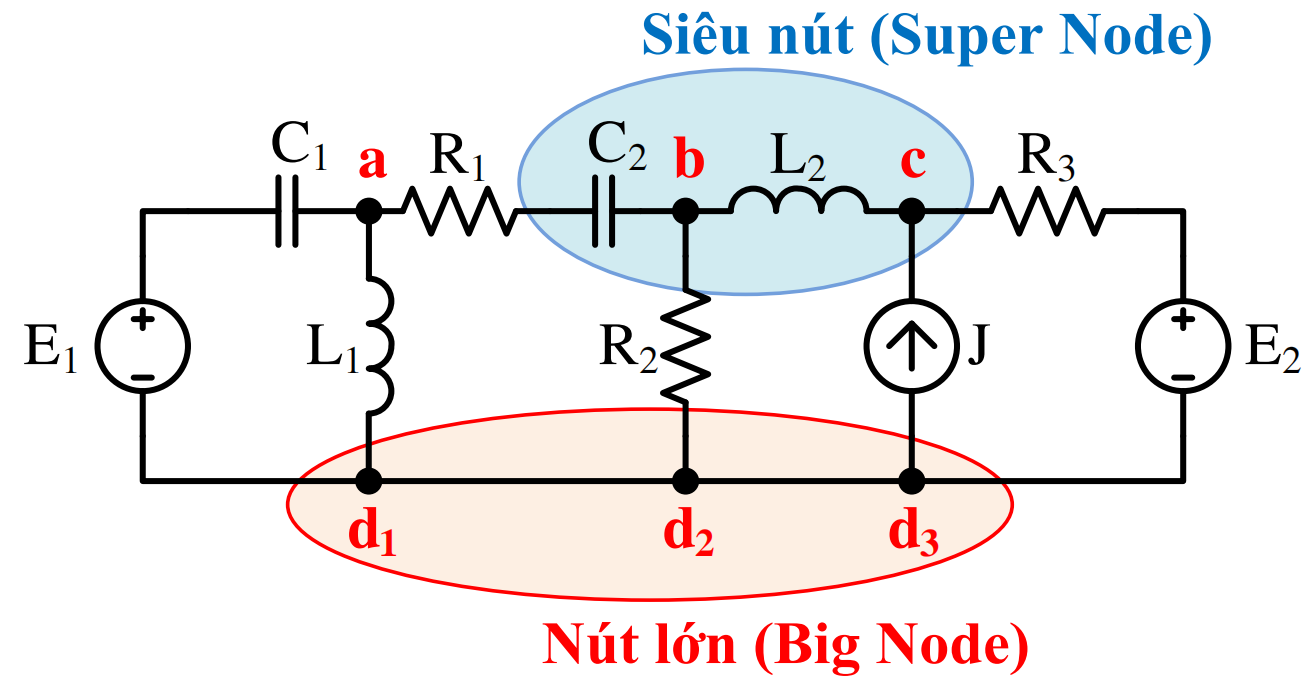
\includegraphics[width = 0.45\textwidth]{./image/15.png}
\end{center}
\subsection{Định luật Kirchhoff 1: KCL (Kirchhoff Current Law)} 
\begin{equation}
  \sum_{k=1 \ (\text{nút})}^{n} \pm i_k = 0
\end{equation}
Qui ước:
\begin{itemize}
  \item Dòng điện đi vào nút giá trị dương.
  \item Dòng ra khỏi nút mang giá trị âm.
\end{itemize}
\begin{center}
  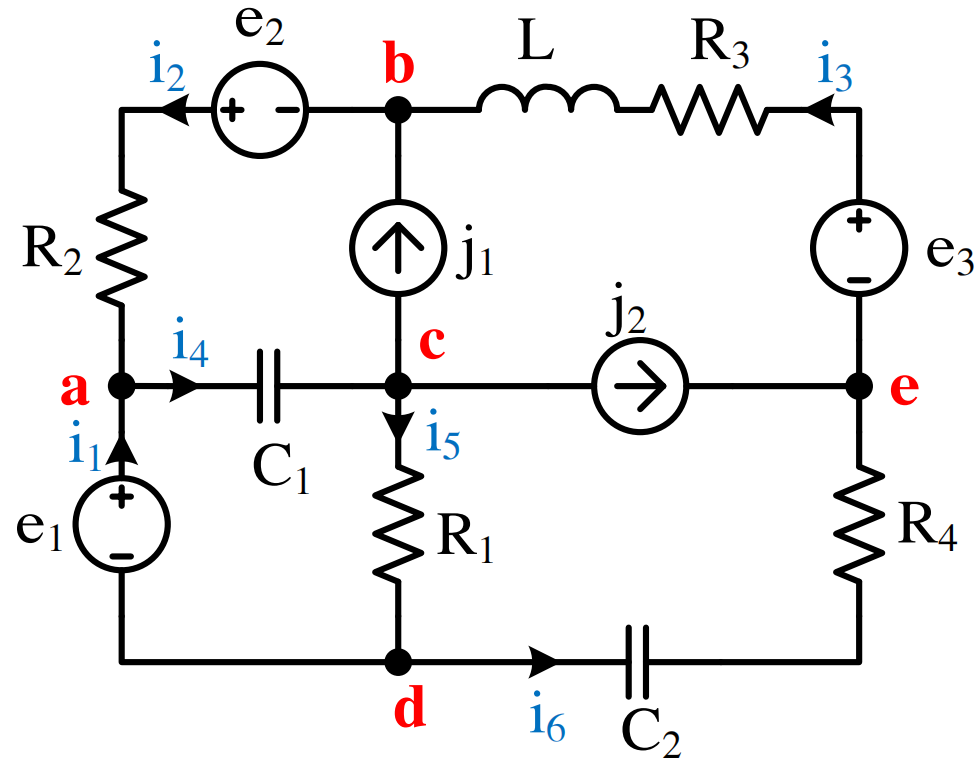
\includegraphics[width = 0.45\textwidth]{./image/16.png}
\end{center}
\subsection{Định luật Kirchhoff 2: KVL (Kirchhoff Voltage Law)} 
\begin{equation}
  \sum_{k=1 \ (\text{vòng})}^{n} \pm u_k = 0
\end{equation}
Qui ước:
\begin{itemize}
  \item Điện áp dương khi cùng chiều vòng.
  \item Điện áp âm khi ngược chiều vòng.
\end{itemize}
\begin{center}
  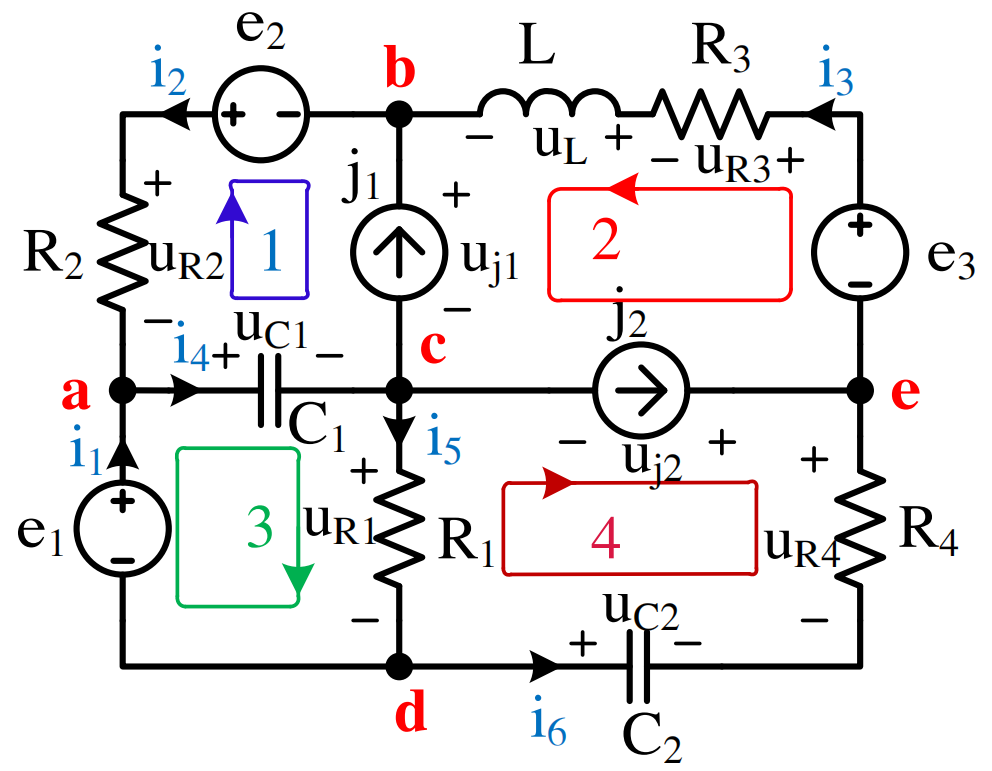
\includegraphics[width = 0.45\textwidth]{./image/17.png}
\end{center}
\subsection{Hệ PT dòng điện nhánh}
\begin{center}
  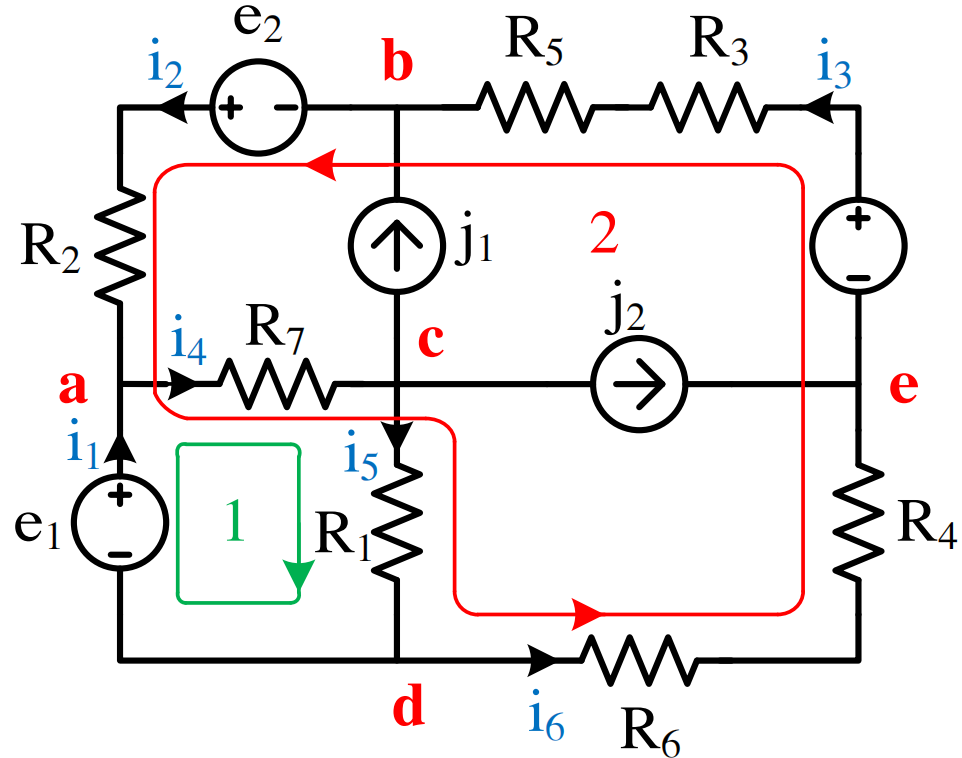
\includegraphics[width = 0.4\textwidth]{./image/18.png} 
\end{center}
Trong đó:\begin{itemize}
  \item d: số nút
  \item n: số nhánh
  \item k: số nguồn dòng
\end{itemize}
(ẩn số là dòng điện trong các nhánh):
\begin{itemize}
  \item d-1: phương trình từ KCL.
  \item n-d+1-k: phương trình từ KVL.
\end{itemize}
\subsection{Biến đổi nguồn áp lý tưởng:}
\begin{equation}
  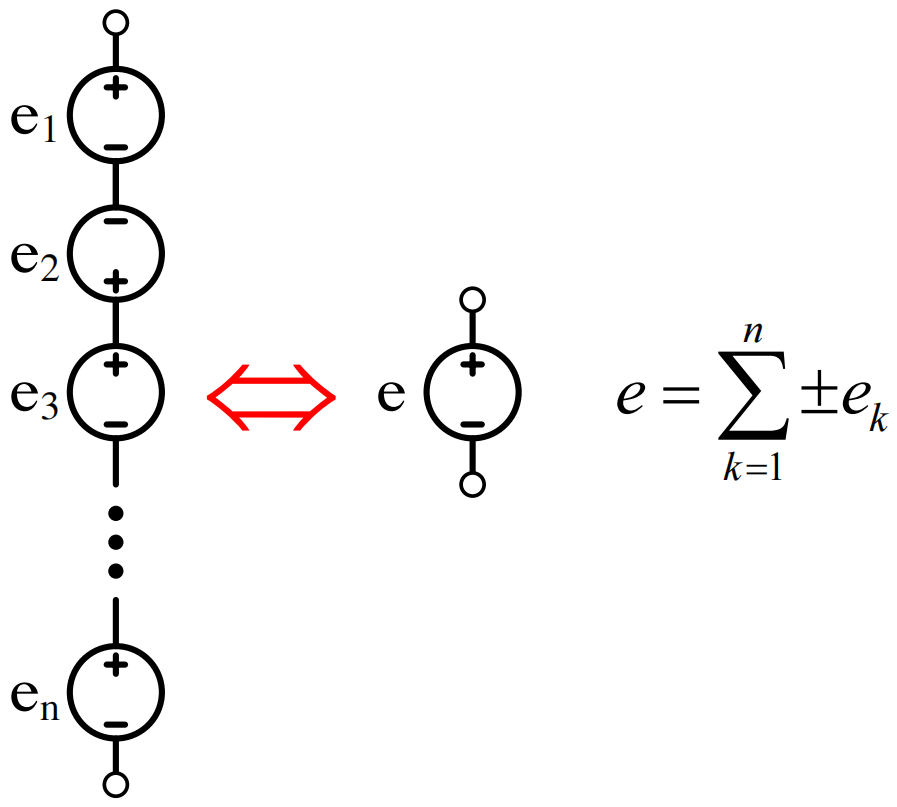
\includegraphics[width = 0.5\textwidth]{./image/19.png}
\end{equation}
\begin{equation}
  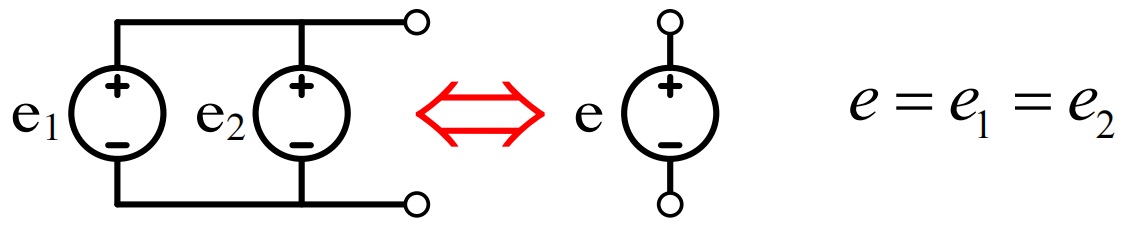
\includegraphics[width = 0.6\textwidth]{./image/20.png}
\end{equation}
\textcolor{red}{Lưu ý:} không tồn tại khi $e_1 \neq e_2$.
\subsection{Biến đổi nguồn dòng lý tưởng:}
\begin{equation}
  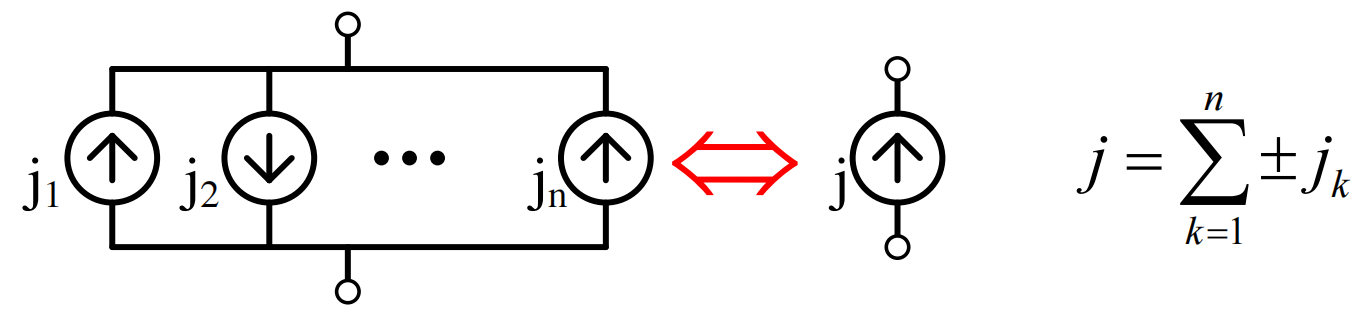
\includegraphics[width = 0.7\textwidth]{./image/21.png}
\end{equation}
\begin{equation}
  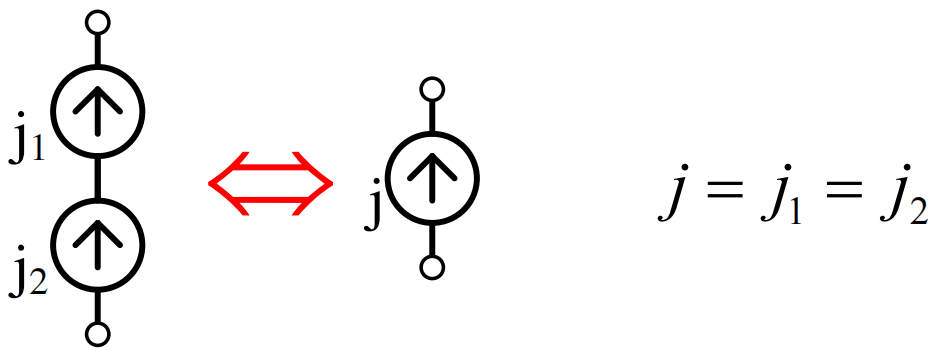
\includegraphics[width = 0.6\textwidth]{./image/22.png}
\end{equation}
\textcolor{red}{Lưu ý:} không tồn tại khi $j_1 \neq j_2$.
\subsection{Biến đổi nguồn thực:}
\begin{center}
  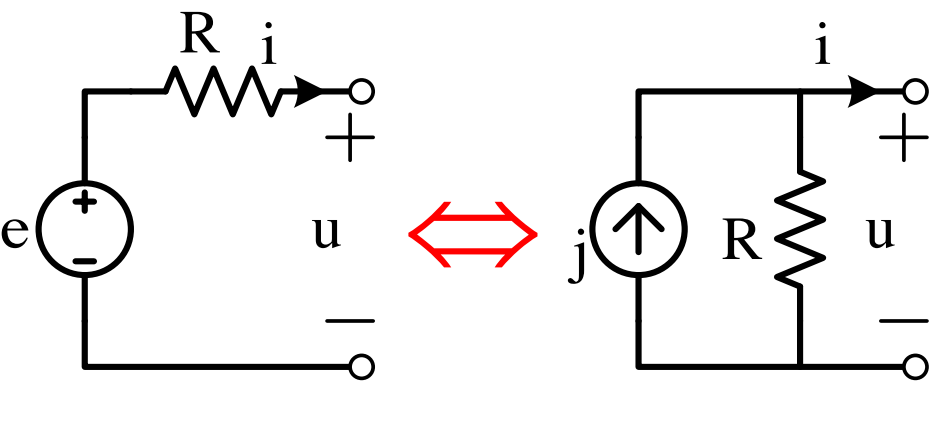
\includegraphics[width = 0.5\textwidth]{./image/23.png}
\end{center}
\begin{equation}
  e=R.j
\end{equation}
\subsection{Biến đổi điện trở nối tiếp:}
\begin{equation}
  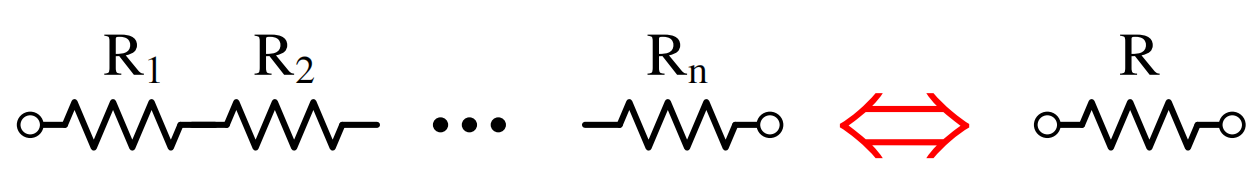
\includegraphics[width = 0.6\textwidth]{./image/24.png} \qquad R = \sum_{k=1}^{n}R_k
\end{equation}
\subsection{Biến đổi điện trở nối tiếp:}
\begin{equation}
  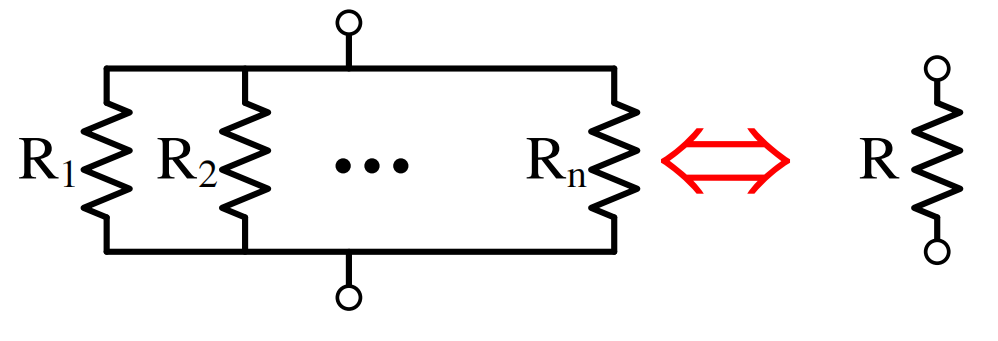
\includegraphics[width = 0.6\textwidth]{./image/25.png} \qquad \frac{1}{R} = \sum_{k=1}^{n}\frac{1}{R_k}
\end{equation}
\subsection{Biến đổi điện trở mắc sao $\leftrightarrow$ tam giác:}
\begin{center}
  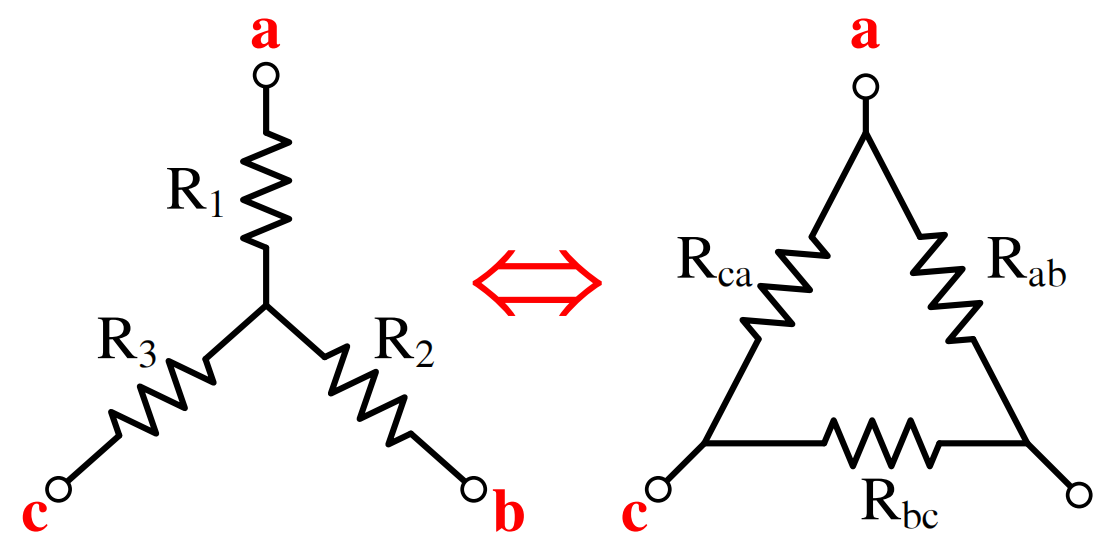
\includegraphics[width = 0.6\textwidth]{./image/26.png}
\end{center}
\begin{equation}
  R_{Y(node)} = \frac{R_{\Delta 1}R_{\Delta 2}(to-node)}{R_{ab}+R_{bc}+R_{ca}} \qquad R_{\Delta} \frac{R_1R_2 + R_2R_3 + R_3R_1}{R_Y (facing - node)}
\end{equation}
\subsection{Quy tắc phân áp:}
\begin{center}
  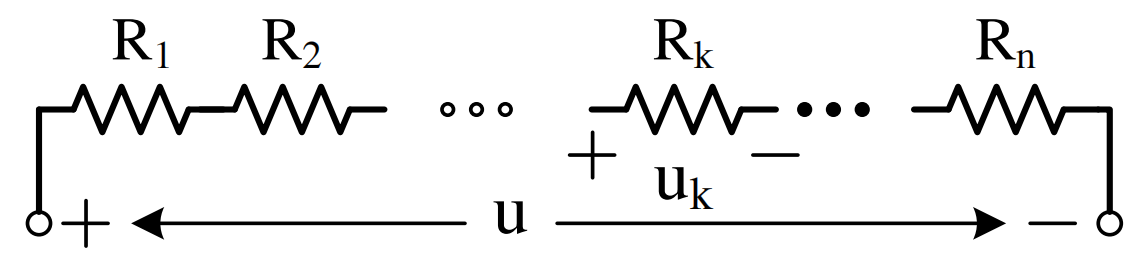
\includegraphics[width = 0.7\textwidth]{./image/27.png}
\end{center}
\begin{equation}
  u_k = \left( \frac{R_k}{\sum R} \right)u
\end{equation}
\subsection{Quy tắc phân dòng:}
\begin{center}
  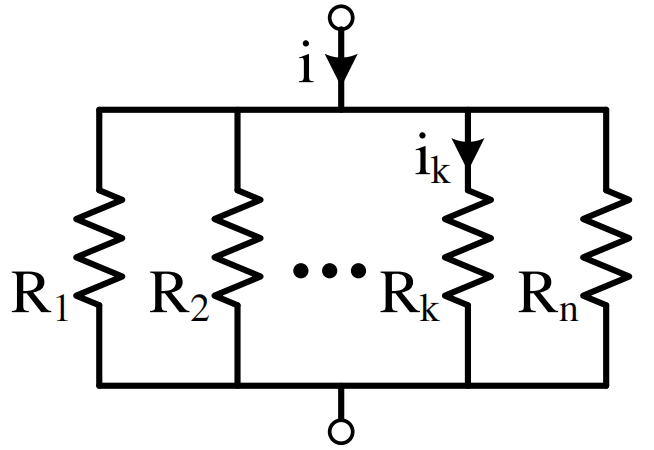
\includegraphics[width = 0.5\textwidth]{./image/28.png}
\end{center}
\begin{equation}
  i_k = \left( \frac{\dfrac{1}{R_k}}{\sum \dfrac{1}{R}} \right)i
\end{equation}